\chapter{Methods}
In this section we explore different methods for reconstructing the 3D scene of hospital and carehome video sequences. We approach this by first considering the 3D environment of the hospital and care home rooms, using current state-of-the-art monocular depth estimation models for extracting point clouds of the rooms. Combining the point clouds with given segmentation labels enables isolation and fitting of the floor plane to be used in estimating the camera extrinsics and thereby aligning the scenes in a shared global coordinate system. We then move on to restoring the people and their motion in the scene by qualitatively comparing regression- and optimization-based human pose estimation methods. % In addition, we explore the use of motion diffusion models for motion extraction, by guiding the generation process in a classifer-guided manner to align the 2D joint projections with labelled keypoints.

Finally, we present our own motion diffusion model trained with classifier-free guidance for text conditioned multi-human motion generation, simplifying the architecture of InterGen by treating the pose embeddings with a learned identity encoding, enabling flexible generation of multi-human interactions. In evaluating its motion generation capabilities with MDM and InterGen, we compare both motion quality (FID score), diversity and multi-modality against the InterGen and MDM models using established evaluation methods.


\section{Restoring 3D Environment}
% TODO: Write here
\begin{figure}
    \centering
    \begin{subfigure}[b]{0.4\textwidth}
        \includegraphics[width=\linewidth]{figures/floor.png}
        \label{fig:floor-mask}
        \caption{Example of floor segmentation mask.}
    \end{subfigure}
    \hfill
    \begin{subfigure}[b]{0.5\textwidth}
        \includegraphics[width=\linewidth]{figures/depth.pdf}
        \caption{Upscaled metric depth map.}
    \end{subfigure}
\end{figure}

Explicitly reasoning about scenes in their physical native 3D dimensions compared to 2D image projections provides a more accurate understanding of spatial relationships and object interactions. One example is much more robust handling of occlusions, as objects that appear occluded in a 2D image can often be separated and distinguished when considering the depth dimension. In general, considering the 3D dimensionality of objects makes it easier to encode priors over ambigious 3D locations from their given 2D projections.


We combine both metric and relative variants of the Depth Anything model (\cite{depthanything}) to restore the depth of the scene. Using the low-resolution 384x512 metric depth predictions, $m_{1:K}$, we restore the scaling and offset from the higher resolution predicted disparity maps, $d_{1:K}$, by linearly fitting the disparity scaling $\alpha$ and offset $\beta$ according to $\argmin \alpha \cdot d_{1:K} + \beta - 1 / m_{1:K}$ for all $K$ key frames to get our upscaled metric depths, $m^*_{1:K} := 1 / (\alpha \cdot d_{1:K} + \beta)$.


\label{section:floor-plane}
\begin{figure}[H]
    \centering
    \includegraphics[width=\linewidth]{figures/rotation.pdf}
    \caption{Translation and rotation of room point cloud aligning the floor with the XY-plane.}
    \label{fig:rotate-floor-planes}
\end{figure}
Using the floor segmentation masks we isolate the floor point cloud and use the outlier robust RANSAC regressor with inline threshold of 5cm to fit the plane equation:

\begin{equation}
    z = \beta_z + \beta_x x + \beta_y y
\end{equation}

To compute the rotation matrix that aligns the normal vector $\hat{\vect{n}}_\text{floor} = \vect{n}_\text{floor} / \| \vect{n}_\text{floor} \|$ (where $\vect{n}_\text{floor} = (0, 1, b_y)^T \times (1, 0, b_x)^T$) of the floor plane in the camera coordinate system with the normal vector $\vect{n}_{XY} = (0, 0, 1)$ of the XY-plane, we can utilize Rodrigues' rotation formula. 

First, we construct the skew-symmetric matrix $\mathbf{K}$ from the components of the cross product vector $\vect{v} = \hat{\vect{n}}_\text{floor} \times \vect{n}_{XY}$. The skew-symmetric matrix $\mathbf{K}$ is defined as:

\begin{equation}
    \mathbf{K} = \begin{bmatrix}
        0 & -v_3 & v_2 \\
        v_3 & 0 & -v_1 \\
        -v_2 & v_1 & 0
    \end{bmatrix}
\end{equation}

Next, we compute the rotation matrix $\mathbf{R}$ using Rodrigues' rotation formula. The formula incorporates the identity matrix $\mathbf{I}$, the skew-symmetric matrix $\mathbf{K}$, and a scaling term based on the angle between the vectors. The resulting rotation matrix is given by:

\begin{equation}
    \mathbf{R} = \mathbf{I} + \mathbf{K} + \mathbf{K}^2 \left(\frac{1 - c}{s^2}\right)
\end{equation}

Here, $\mathbf{I}$ is the identity matrix, $c$ is the dot product of $\mathbf{a}$ and $\mathbf{b}$, and $s$ is the norm of the cross product vector $\mathbf{v}$. This formula ensures that the rotation matrix $\mathbf{R}$ not only aligns $\mathbf{a}$ with $\mathbf{b}$ but also preserves the orthogonality and orientation of the coordinate system.

Finally, we transform the point cloud by translating it to align the floor plane intercept with the origin, followed by rotating it using the computed rotation matrix:

\begin{equation} \label{eq:transform-points}
    \vect{p}^* = \mathbf{R} \left(\vect{p} - (0, 0, b_z)^T \right) 
\end{equation}
In a similar fashion, we transform our poses by applying \cref{eq:transform-points} to our pose root joint translations. Since our joint rotations are relative to the root global orientation, $\mathbf{O}$, we first compute its inverse global-to-local rotation matrix, $\mathbf{O}^{-1}$. After applying the new rotation matrix $\mathbf{R}$, we then invert the result to convert back from local-to-global orientation:

\begin{equation} % TODO: Check this. Isn't this just taking the transpose since orthogonal matrices?
    \mathbf{O}^* = \left(\mathbf{R} \mathbf{O}^{-1} \right)^{-1}
\end{equation}
The resulting transformation of the point cloud and poses in aligning the floor with the XY-plane is illustrated in \cref{fig:rotate-floor-planes}.


% Our two baseline pose estimation methods consists of the regression-based HMR2.0 pose estimation model 
%to labeled bounding boxes of people in the frame as well as regression-based SMPLify method. We compare this with a novel


% \section{Tracking \& Matching}
% We track the predicted staff and patients across multiple frames, indicated by $t = 1 \ldots T$, by iteratively assigning the predictions, $\{ P_i^{(t)} \}_{i=1}^{M_t}$, to the latest known tracks, $\{ Q^{(t)}_{j} \}_{j=1}^{N_t}$ by greedily picking the assignment with the minimum cost:
% \begin{equation}
%     \argmin_{i,j} \mathcal{L}_\text{track}(P^{(t)}_i, Q^{(t-1)}_j),
% \end{equation}
% until either all predictions or latest tracks have been assigned exactly once. In the case of any unassigned predictions, a new track is initialized. After tracks have been assigned, the latest track $Q^{(t)}_j$ is updated with the assigned predictions. We choose the following composite loss function:
% \begin{equation}
%     \mathcal{L}_\text{track}(P, Q) = \alpha \norm{P_\text{3D kpts} - Q_\text{3D kpts}}{2} + \beta \norm{P_\text{class} - Q_\text{class}}{\infty},
% \end{equation}
% incorporating both the Euclidean distance between the 3D joint keypoints as well as the predicted person class (staff/patient), with $\alpha$ and $\beta$ weighting the influence of each term. The tracks, $T_i$, are then greedily matched to the ground truth annotations $G_j$, minimizing the loss:
% \begin{equation}
%     \mathcal{L}_\text{match}(T, G) = \sum_t^{T} \begin{cases}
%         \norm{a^{(t)}_{\text{track}, \text{2D kpts}} - b^{(t)}_{\text{track}, \text{2D kpts}}}{2} & \text{if}\ a^{(t)}_\text{track} \in a_\text{track} \\
%         \gamma & \text{otherwise}
%     \end{cases}
% \end{equation}
% over the trajectory time horizon $t = 1,2,\ldots,T$ where $\gamma$ is the punishment for not detecting the person.

\section{Restoring Human Motion}
% TODO: Write this

\subsection*{Regression-based Pose Estimation} \label{section:regression-pose-estimation}
\begin{figure}[H]
    \centering
    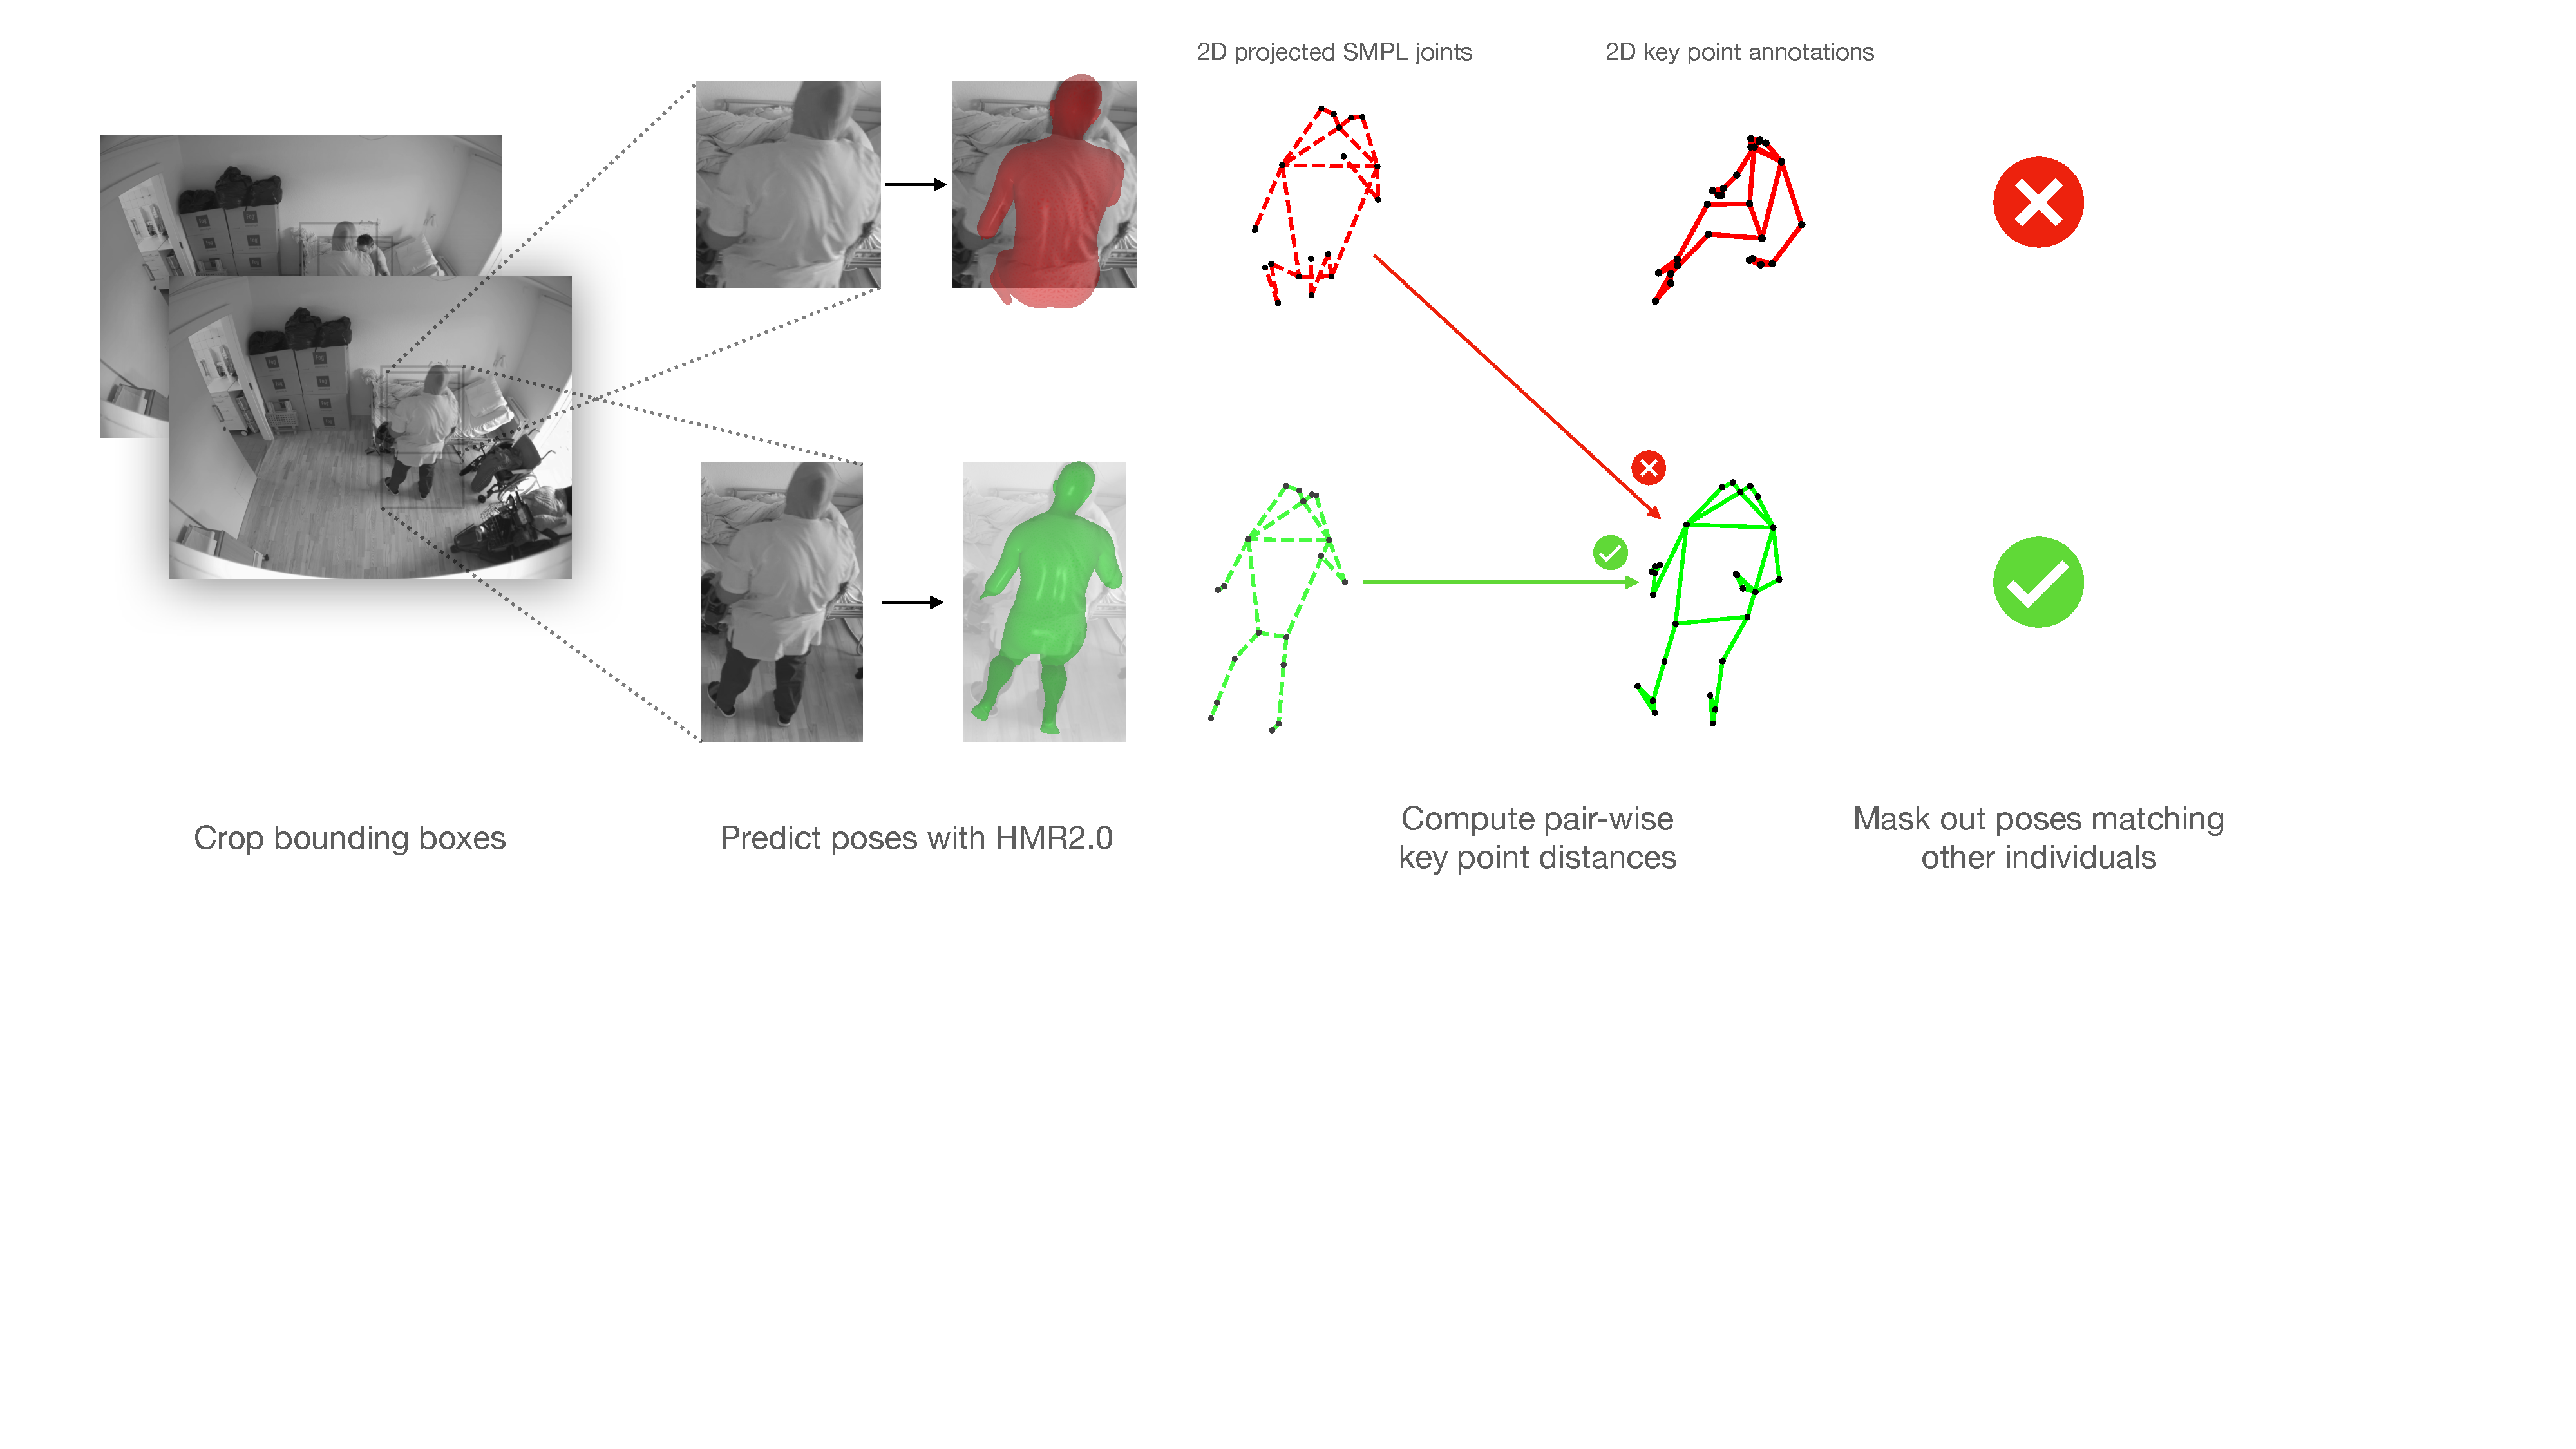
\includegraphics[width=\linewidth]{figures/pose-extraction.pdf}
    \caption{Illustration of pose extraction process with occlusion handling.}
    \label{fig:pose-extraction}
\end{figure}
We leverage the pretrained HMR2.0 model from \cite{goel2023humans} for pose extraction, applying it frame-wise to crops of each human bounding box in the frame. This approach ensures proper alignment with existing dataset annotations without the need for additional tracking. To handle potential occlusions that may cause duplicate predictions of the occluding pose, pairwise euclidean keypoint distances are computed for all edges in the bipartite graph of annotated 2D keypoints and SMPL joint 2D projections for individuals in the current frame. Poses with the minimum keypoint distance to other individuals' annotated keypoints are masked out.

\subsection*{Smoothing poses}
Due to poses being predicted independently per frame, the combined pose sequences often lack temporal consistency, resulting in janky or erratic movements. To address this issue, we refine the pose sequences by optimizing for smooth trajectories across all $1 \dots T$ frames by minimizing a composite smooth loss objective assuming constant velocity:

\begin{equation} \label{eq:smooth-motion}
    \mathcal{L}_\text{smooth} = \sum_t{\| \hat{\vect{j}}^{(t)} - \vect{j}^{(t)} \|_2} + \lambda_{\hat{j}} \sum_t{\mathcal{R}_{\bar{j}}^{(t)}}
\end{equation}

where $\hat{\vect{j}}^{(t)} = \vect{j}^{(t-1)} + \vect{v}^{(t-1)}$ is the predicted joint location at time $t$ assuming constant velocity $\vect{v}^{(t)} = \vect{j}^{(t)} - \vect{j}^{(t-1)}$, and $\mathcal{R}_{\bar{j}}^{(t)} = \| \vect{j}^{(t)} - \bar{\vect{j}}^{(t)} \|_2$ a regularization term preventing the optimized location $\mathbf{j}^{(t)}$ to not diverge too far from the initially predicted joint location $\bar{\vect{j}}^{(t)}$.


\section{Optimization-based pose estimation from keypoints}
As baseline optimization-based method, the SMPLify-X framework is naively to the temporal dimension by introducing a smooth loss objective, as previously defined in \cref{eq:smooth-motion}. This extension relates sequences of keypoints over time, ensuring a coherent reconstruction of 3D motion. 

We jointly optimize the translation, root orientation, body pose and shape as well as the 2D keypoint reprojection error, driving the motion. The overall objective function is formulated as follows:
\begin{equation}
    \mathcal{L}_{\text{total}} = \lambda_{\text{kpts}} \mathcal{L}_{\text{kpts}} + \lambda_{\text{pose}} \mathcal{L}_{\text{pose}} + \lambda_{\text{shape}} \mathcal{L}_{\text{shape}} + \lambda_{\text{smooth}} \mathcal{L}_{\text{smooth}}
\end{equation}
where $\lambda_\text{kpts}$,  $\lambda_\text{pose}$,  $\lambda_\text{shape}$ and  $\lambda_\text{smooth}$ again are hyperparameters weighing the contributions of each loss factor. The keypoint loss is given by:
\begin{equation} \label{eq:kpts-error}
    \mathcal{L}_\text{kpts} = \mathbb{E}_{i,t} \| \mathcal{P}( \vect{K} \vect{j}_{\text{3D},i}^{(t)}) - \vect{j}_{\text{2D},i}^{(t)} \|_2^2
\end{equation}
with $\vect{K}$ being our camera intrinsics and $\mathcal{P}$ is the perspective projection function. Joint locations are computed by forward-kinematics of the joint angles (\cref{eq:smpl-joints}) and are thus guaranteed to satisfy anatomical constraints. 

We represent the root body orientation using a 6D representation in favor of Euler angles, axis angles and quarternions, as they have been shown to be continuous and neural network friendly (\cite{Zhou_2019_CVPR}), while being easy to convert to and from rotation matrices. As both body pose, $\vect{z}^{(t)}$, and body shape vectors, $\vect{\beta}$, are normally distributed latent representations, preventing implausible body poses and shapes simply becomes a matter of regularizing their magnitudes. We choose an L2 loss for this:
\begin{equation}
    \mathcal{L}_\text{pose} = \sum_t \| \vect{z}^{(t)} \|_2^2, \quad \mathcal{L}_\text{shape} =  \| \vect{\beta}^{(t)} \|_2^2 
\end{equation}



% \section{Keypoint-Guided Motion Diffusion}
% We investigate whether motion diffusion can be utilized in extracing the 3D motion from 2D keypoint annotations with the hypothesis that the model will function as a good motion prior. Preferably, the joints in the generated motion should map well the 2D keypoint annotations, but still satisfy the properties of plausible motion. To steer the model towards generating keypoint consistent motion, we make use of classifier guidance, by introducing a drift term in the denoising process that pushes the motion in the direction of the projection rays of the keypoints. Specifically, we modify our score function in \cref{eq:classifier-guidance} by substituting the classifier term with the 2D keypoint reprojection error in \cref{eq:kpts-error} to get:
% \begin{equation}
%     \bar{\vect{\epsilon}}_{\theta}(\vect{x}_t, t) = \vect{\epsilon}_\theta(\vect{x}_t, t) - \sqrt{1 - \bar{\alpha}_t} \grad_{\vect{x}_t} \mathcal{L}_\text{kpts}(\vect{x}_t, \vect{J})
% \end{equation}
% As our motion diffusion model generates motion in the world coordinate system, we first estimate the camera pose by aligning the floor with the XY-plane as in \cref{section:floor-plane}.

% \section{Multi-human Motion Diffusion Model}
% \begin{figure}[H]
%     \hspace*{-1cm}
%     \includegraphics[width=\linewidth+1cm]{figures/diffusion-model.pdf}
%     \caption{Architecture of our proposed Multi-Human Motion Diffusion model.}
%     \label{fig:diffusion-model}
% \end{figure}
% Due to its static dual-denoising architecture, the Intergen model is inherently limited in only supporting generations of exactly two person interactions. We investigate relaxing this constraint by instead employing a generic transformer encoder as denoisning network operating on the flattened motion sequence. As this results in the model loosing its inductive bias, we treat each pose encoding, $\vect{x}_i$, with a learned identity embedding to help the model differentiate between multiple people. At each denoising step, the model samples without replacement one of $\mathcal{I}$ unique identity embedding per person and adds this to all pose embeddings for that individual. We include the same loss functions as InterGen, but adapt these for N-way pairwise comparison. The model is trained using classifer-free guidance, by masked out the description embedding 10\% of the time. An illustration of the model is seen in \cref{fig:diffusion-model}. 






% We use the notation
% \vect{J} for all joints at all times
% \vect{J}^{(1)}_t all joints for person one at time t
% \vect{j}^{(j)}_i joint i at time t (for all people)



%We steer the diffusion process

%at test time using classifier guidance

% by computing gradient of the keypoint loss 
% TODO: Write something about the annotations in the Teton data section.

% TODO: We are assuming that the relative doesn't change dynamic range during the scene (which might be wrong). Save for discussion.


% We utilize pseudo ground truth disparity maps generated by the Depth Anything model, inversely proportional to the scene depth, in order to reconstruct a point cloud of the scene. To recover the depth scale and offset we rasterize the predicted SMPL poses, extract the z-buffer, compute the inverse depth and regress the intersection with the normalized disparity maps using the Random Sample Consensus (RANSAC) algorithm robust to outliers. 

% \begin{equation}
%     \begin{bmatrix}p
%         x \\ y \\ 1/z \\ 1
%     \end{bmatrix} = \begin{bmatrix}
%         f_x & 0 & 0 & p_x \\
%         0 & f_y & 0 & p_y \\
%         0 & 0 & 1 & 0 \\
%         0 & 0 & 0 & 1
%     \end{bmatrix} \begin{bmatrix}
%         X \\ Y \\ Z \\ 1
%     \end{bmatrix}
% \end{equation}


% \begin{equation}
%     X = \frac{Z}{f_x} \left( x - p_x \right) , \quad Y = \frac{Z}{f_x} \left(y - p_y \right)
% \end{equation}
% where $f_x$, $f_y$ are the horizontal and vertical focal lenghts respectively and ($p_x$, $p_y$) is the principal point often chosen as the center $(w/2,h/2)$ of the image. 


% Something about using the original poses + vPoser (human pose prior) + annotated keypoints.
% TODO: Write this?


% \section{Unification of datasets}
% Before concatenating the HumanML3D, InterHuman and our own Teton dataset we make sure they all conform to the same coordinate system and scaling by implicitly representing the floor as the XY-plane with positive Z indicating the upwards direction using metric units for coordinates. This removes the need to explicitly condition the model on the floor plane possibly simplifying the learning task for more efficient training.


% \section{Motion and scene representation}


% We follow the work by \cite{liang2024intergen} and represent each pose in the motion sequence using their proposed non-canonical representation, but disregard the binary foot-ground contact features:
% \begin{equation}
%     \vect{x}_t = \left[\vect{j}_g^p,\ \vect{j}_g^v,\ \vect{j}^r \right]
% \end{equation}
% where $\vect{j}_g^p$ are the global joint positions, $\vect{j}_v^p$ the global joint velocities and $\vect{j}^r$ the relative SMPL 6D joint rotations.


% Previous work on single human motion generation uses a canonical representation 

% We use a 6D continuous representation of the joint angles as according to \cite{Zhou_2019_CVPR}.
% We represent the motion similar to 

% TODO: Write about 6D representations


% \section{Diffusion model}


% otion data for each person is flattened into a single array of poses. Each pose in the sequence is embedded using a linear layer. To embed the motion timestamp, we add positional encoding to the latent variables ($z_t$).

% Identity encoding is achieved by randomly selecting (without replacement) a learned ID embedding for each person and adding it to each pose embedding. Additionally, class information (such as medical staff, patients, etc.) is encoded by adding a learned class embedding.

% For textual descriptions, we use the CLIP model to encode the text, and the resulting output is embedded using a linear layer. This embedded text is then prepended to the input sequence for the transformer.

% Object point clouds are processed by clustering the coordinates into groups of 64, which are then embedded using a linear layer. These embeddings are integrated into the model to provide spatial context.




% TODO define loss functions